\section{Prediction for unassociated sources in 3FGL and comparison with 4FGL}
\lb{sec:3FGLprediction}


In this section we use the algorithms from the previous section to predict classes for the unassociated sources in the 3FGL. 
We have selected RF with 50 trees and max depth of 6, BDT with 100 trees and max depth of 2, NN with 10 neurons, ADAM solver, 300 epochs, and LR with LBFGS solver, 200 iterations.
The details of the selected algorithms are summaries in Table \ref{tab:selected_algs}.
``Average testing accuracy" is computed by taking 1000 times 70\% - 30\% split into training testing samples and averaging over the 
accuracies computed for the testing samples.
In addition, we look at sources, which are unassociated in 3FGL but have either pulsar or AGN association in 4FGL: there are 242 such sources.
The accuracy of our prediction for the four selected algorithms, taking the 4FGL classes as the true values, is reported in the column ``Accuracy from Comparison with 4FGL''.
The correct classifications and misclassifications for the 242 sources with associations in 4FGL are also presented in Figure \ref{fig:Maps_data}.


\begin{table}[!h]

\resizebox{0.45\textwidth}{!}{
    \tiny
 %  \centering
    \renewcommand{\tabcolsep}{0.3mm}
\renewcommand{\arraystretch}{1.5}

    \begin{tabular}{|c|c|c|c|}
    \hline
    Algorithm&Parameters & Average  & Accuracy from \\
    & & Testing Accuracy & Comparison with 4FGL\\
    \hline
    RF& 50 trees, max depth 6  &97.42& 97.19  \\
    \hline %\midrule   -> aakash do you mean this?
    BDT & 100 trees, max depth 2    &   97.80&96.28 \\
%    \hline %\midrule   -> aakash do you mean this?
%    BDT & 200 trees, max depth 2    &   95.8  \\
    \hline
    NN & 300, 10 Neurons, Adam & 97.40& 95.65 \\
    \hline
    LR & LBFGS solver, 200 iterations & 97.60& 95.09 \\
    \hline
     
    \end{tabular}}
    \vspace{0.2cm}
    \caption{Accuracy of the 4 selected algorithms on 3FGL unassociated data.}
    \label{tab:selected_algs}
\end{table}

Here we discuss the results of our probabilistic classification on the unassociated data. The 242 sources for whom FGL counterparts existed were plotted in figure 10. This figure shows all AGNs and PSRs, including those which were correctly or incorrectly identified by all the 4 algorithms (given by keyword only) and those which are a mix of correct and incorrect classification by at least one of the 4 algorithms (given by keywords either/or). 
\begin{figure*}[h]
\centering
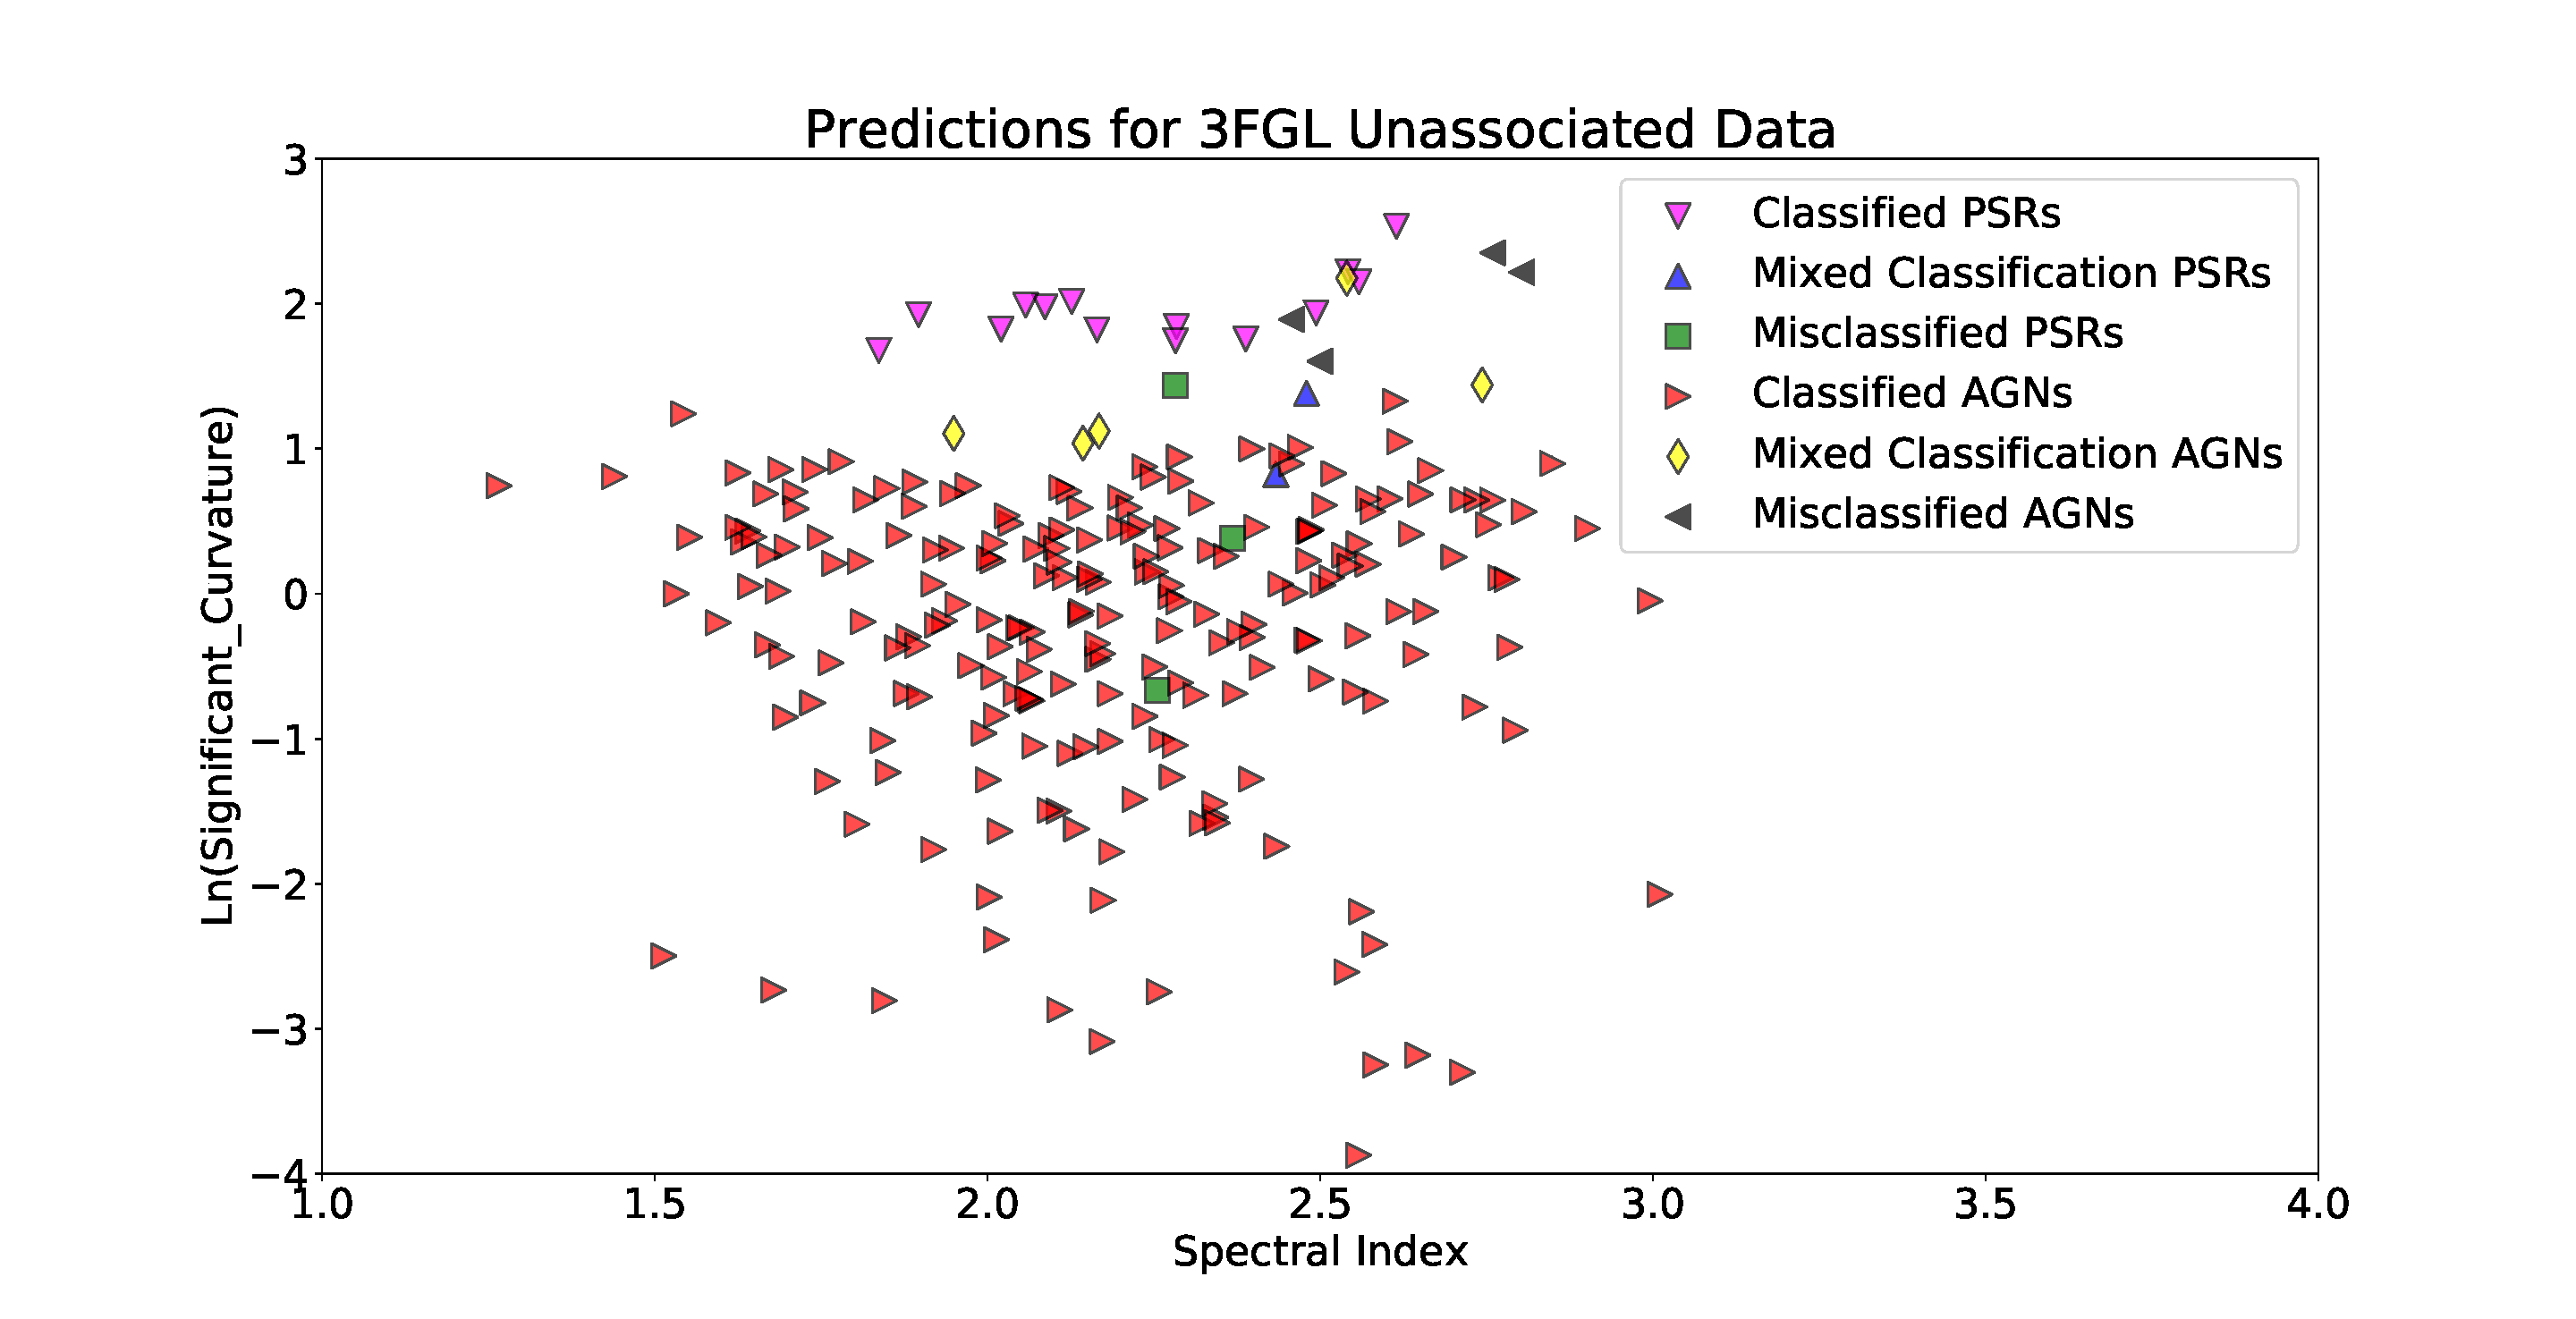
\includegraphics[width=\textwidth]{plots/plot_final.pdf}
%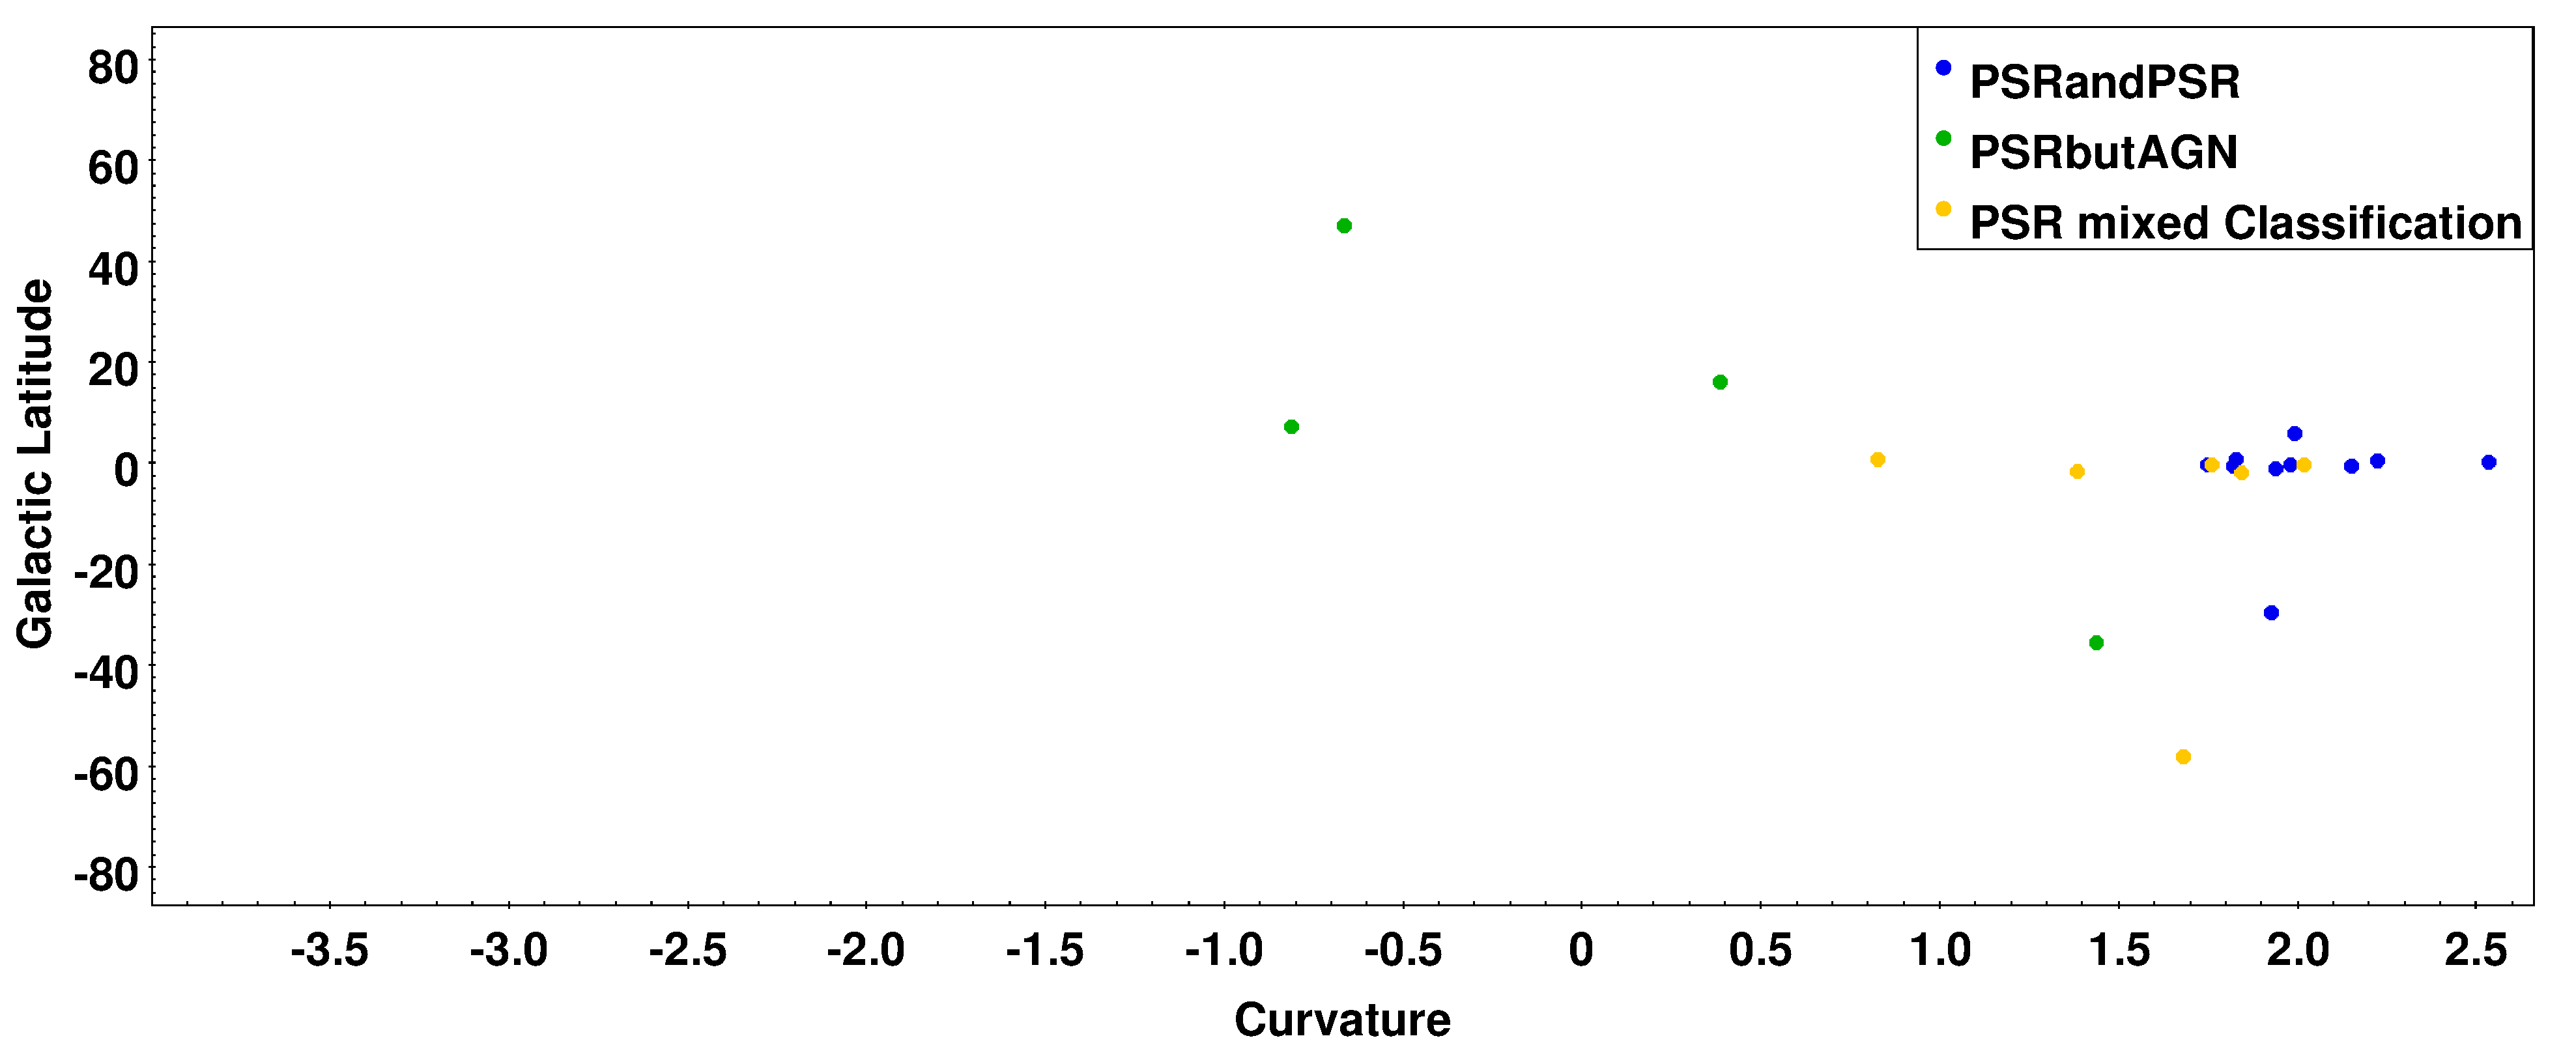
\includegraphics[width=\twopicsp\textwidth]{plots/PSR3.pdf}
\caption{Comparison of class prediction for unassociated 3FGL sources with classes in 4FGL. }
%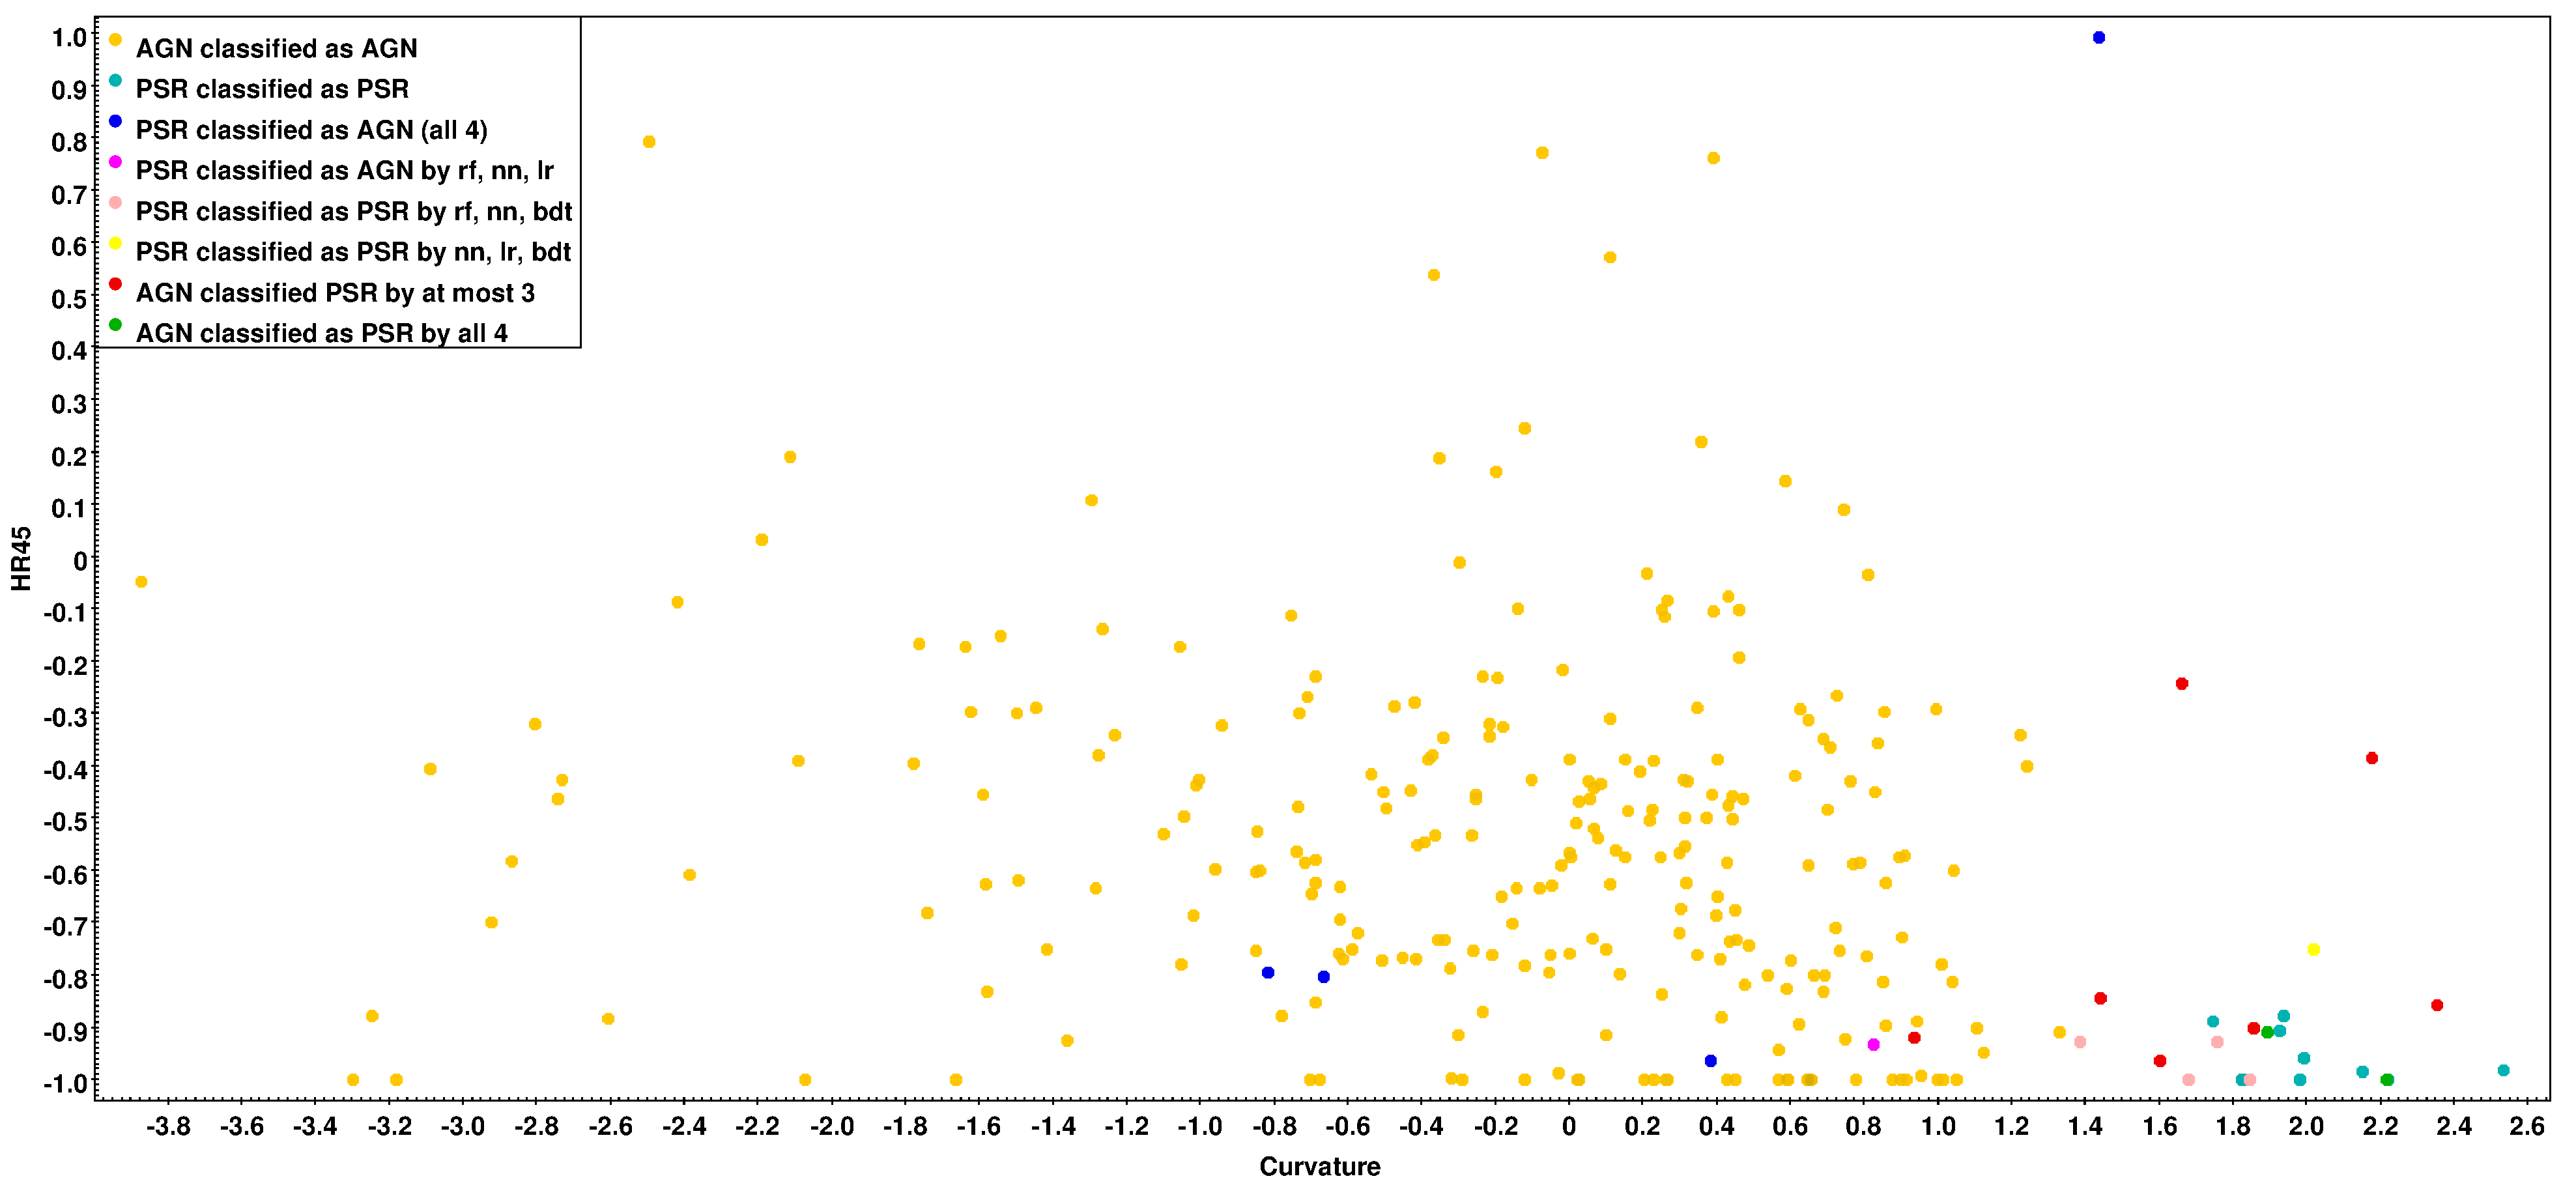
\includegraphics[width=\twopicsp\textwidth]{plots/final_catalog.pdf}
\label{fig:Maps_data}
\end{figure*}

Table 4 shows an example of the probabilistic catalog we created for these 242 sources.

\pgfplotstableread[col sep=comma]{data/catalogs/3FGL_unassoc_vs_4FGL_assoc.csv}\loadedtable
\begin{table}
\pgfplotstabletypeset[columns={Source_Name_3FGL,AGN_BDT,AGN_RF,AGN_LR,AGN_NN},
column type=l,
string type,
every head row/.style={before row={\toprule & \multicolumn{4}{c}{AGN Probability} \\},after row=\midrule,},
every last row/.style={after row=\vdots },
columns/Source_Name_3FGL/.style={column name=Source Name},
columns/AGN_BDT/.style={column name=BDT,numeric type,fixed,precision=3},
columns/AGN_NN/.style={column name=NN,numeric type,fixed,precision=3},
columns/AGN_RF/.style={column name=RF,numeric type,fixed,precision=3},
columns/AGN_LR/.style={column name=LR,numeric type,fixed,precision=3},
skip rows between index={4}{242}
]\loadedtable
\caption{Catalog Rows and Columns for 3FGL unassociated data}
\end{table}